%Tipo de Documento [Conferencia]

\documentclass[conference]{IEEEtran}\usepackage[]{graphicx}\usepackage[]{color}
%% maxwidth is the original width if it is less than linewidth
%% otherwise use linewidth (to make sure the graphics do not exceed the margin)
\makeatletter
\def\maxwidth{ %
  \ifdim\Gin@nat@width>\linewidth
    \linewidth
  \else
    \Gin@nat@width
  \fi
}
\makeatother

\definecolor{fgcolor}{rgb}{0.345, 0.345, 0.345}
\newcommand{\hlnum}[1]{\textcolor[rgb]{0.686,0.059,0.569}{#1}}%
\newcommand{\hlstr}[1]{\textcolor[rgb]{0.192,0.494,0.8}{#1}}%
\newcommand{\hlcom}[1]{\textcolor[rgb]{0.678,0.584,0.686}{\textit{#1}}}%
\newcommand{\hlopt}[1]{\textcolor[rgb]{0,0,0}{#1}}%
\newcommand{\hlstd}[1]{\textcolor[rgb]{0.345,0.345,0.345}{#1}}%
\newcommand{\hlkwa}[1]{\textcolor[rgb]{0.161,0.373,0.58}{\textbf{#1}}}%
\newcommand{\hlkwb}[1]{\textcolor[rgb]{0.69,0.353,0.396}{#1}}%
\newcommand{\hlkwc}[1]{\textcolor[rgb]{0.333,0.667,0.333}{#1}}%
\newcommand{\hlkwd}[1]{\textcolor[rgb]{0.737,0.353,0.396}{\textbf{#1}}}%

\usepackage{framed}
\makeatletter
\newenvironment{kframe}{%
 \def\at@end@of@kframe{}%
 \ifinner\ifhmode%
  \def\at@end@of@kframe{\end{minipage}}%
  \begin{minipage}{\columnwidth}%
 \fi\fi%
 \def\FrameCommand##1{\hskip\@totalleftmargin \hskip-\fboxsep
 \colorbox{shadecolor}{##1}\hskip-\fboxsep
     % There is no \\@totalrightmargin, so:
     \hskip-\linewidth \hskip-\@totalleftmargin \hskip\columnwidth}%
 \MakeFramed {\advance\hsize-\width
   \@totalleftmargin\z@ \linewidth\hsize
   \@setminipage}}%
 {\par\unskip\endMakeFramed%
 \at@end@of@kframe}
\makeatother

\definecolor{shadecolor}{rgb}{.97, .97, .97}
\definecolor{messagecolor}{rgb}{0, 0, 0}
\definecolor{warningcolor}{rgb}{1, 0, 1}
\definecolor{errorcolor}{rgb}{1, 0, 0}
\newenvironment{knitrout}{}{} % an empty environment to be redefined in TeX

\usepackage{alltt}

%BIBLIOTECAS

% Este paquete se utiliza para generar texto o graficas de relleno.
%\usepackage{blindtext, graphicx}
%Biblioteca para graficas
\usepackage{graphicx}
%Biblioteca para lectura de caracteres ortográficos (tildes..etc. ) 
\usepackage[utf8]{inputenc}
%Biblioteca para graficos vectrizados.svg 
\usepackage{svg}
\usepackage{enumerate}
%Biblioteca para enumerar figuras tablas.. etc en español 
\usepackage[english]{babel}
\usepackage{hyperref}


%INICIO DEL DOCUMENTO
\IfFileExists{upquote.sty}{\usepackage{upquote}}{}
\begin{document}


% TITULO DEL PAPER
\title{Data analysis of the Online Retails DataSet}


% NOMBRE DE LOS AUTORES
\author{
 \IEEEauthorblockN{Raul Alejandro Buitrago Castellanos}
 \IEEEauthorblockA{Ingeniero de Sistemas\\ 
  Universidad Distrital Francisco José de Caldas\\
  Bogotá D.C., Colombia\\
  Email: raulhabits@gmail.com}
}

%TITULO
\maketitle

%Iniciar Abstract
\begin{abstract}
 This document contains a data analysis of the ``Online Retail'' dataset provided by the UCI Machine Learning Repository web site, this analysis is made to get knowledge from the transactions described in the dataset through a time line.
\end{abstract} 

%Iniciar Palabras Clave Formato IEEE
\begin{IEEEkeywords}
	Dataset, Data Mining, Big Data Analytics, Business intelligence.
\end{IEEEkeywords}

%SECCIÓN 1. INTRODUCCIÓN 
\section{Introducción}
	El gobierno de Colombia, ha liberado datos de ámbito general donde terceros puedan tener acceso a ellos, los utilicen y generen servicios de perfil social, fortaleciendo así la transparencia de la información gubernamental.
	Las aplicaciones de los resultados de los análisis de los datos abiertos tienen como propósito facilitar la toma de decisiones con mayor certidumbre de forma eficiente.
	En el presente artículo analizaremos datos publicados por el DANE basados en una encuesta realizada en el 2015 donde se representan los resultados a preguntas relacionadas con los aportes al sistema de seguridad social colombiano, los cuales serán abordados en este estudio. El alcance de esta revisión se limitará a dos variables: a) edad, b) Monto de los aportes al sistema de seguridad social Colombiano.
	\\

\section{Datos Abiertos}

Según el Ministerio de Tecnologías de la Información y las Comunicaciones de la República de Colombia MinTIC, los Datos Abiertos son todos aquellos datos primarios, sin procesar, en formatos estándar, estructurados e interoperables que facilitan su acceso y permiten su reutilización, los cuales están bajo la custodia de las entidades públicas y que pueden ser obtenidos y ofrecidos sin reserva alguna, de forma libre y sin restricciones, con el fin que terceros puedan reutilizarlos y crear servicios derivados de los mismos.
\\
Los datos abiertos se caracterizan por lo siguiente:
  \begin{itemize}
  	\item \textbf{Disponibilidad y acceso}: la información debe estar disponible como un todo y a un costo razonable de reproducción, preferiblemente descargándola de internet. Además, la información debe estar disponible en una forma conveniente y modificable.
  	
	\item \textbf{Reutilización y redistribución}: los datos deben ser provistos bajo términos que permitan reutilizarlos y redistribuirlos, e incluso integrarlos con otros conjuntos de datos.
	
	\item \textbf{Participación universal}: todos deben poder utilizar, reutilizar y redistribuir la información. No debe haber discriminación alguna en términos de esfuerzo, personas o grupos. Restricciones “no comerciales” que prevendrían el uso comercial de los datos; o restricciones de uso para ciertos propósitos (por ejemplo sólo para educación) no son permitidos. (Public.Resource.Org, 2007).
	
  \end{itemize}

Los datos abiertos se representan de tal manera que permitan a los diversos países alcanzar sus metas tanto estratégicas como operativas pretendiendo “generar servicios de valor agregado a la sociedad, a través del desarrollo de aplicaciones realizadas por terceros (comunidades de desarrollo, industria infomediaria y academia), que utilizan los datos abiertos generados por las entidades de los diversos Estados”. 

El modelo de datos abiertos definido por el estado colombiano, tiene como principales componentes “los objetivos asociados a la implementación de los mismos en el país,  los principios de diseño en las  diferentes  perspectivas, el  modelo específico  con  los elementos  estratégicos,  tácticos,  operativos  y  de  soporte  y por último, el  mapa  de  ruta que  define  las  acciones  puntuales  a ejecutar para apropiar el modelo de datos abiertos definido”.

Una de las entidades del estado Colombiano que está a la vanguardia en el tema de datos abiertos es el Departamento Administrativo de Estadística DANE, el cual a la fecha ha puesto a disposición de público su información en formato de microdatos o Datos Enlazados, también conocidos como Linked Data LD, los cuales presentan la propiedad de vincularse de manera distribuida en la Web, de tal forma que se pueden referenciar al igual que lo hacen los enlaces de las páginas web (W3C.es, 2012).

Si bien el objeto de este artículo son el análisis de los datos abiertos expuestos por el DANE, actualmente este tema ha evolucionado en Datos Abiertos Enlazados, también conocidos como Linked Open Data LOD, que consisten en la simbiosis de los Datos Abiertos (Open Data) y los Datos Enlazados (Linked Data). 

El consorcio que define los estándares para la web, conocido como W3C, ha publicado en su glosario que los datos abiertos enlazados son un conjunto de datos que se encuentran asociados y disponibles en la Web pública, al igual que cuentan con licenciamiento abierto para su reutilización. La publicación de los datos abiertos enlazados en la web permite realizar consultas distribuidas sobre los conjuntos de datos, (2015e).

A partir del concepto de Datos Abiertos, entre el 7 y 8 de diciembre de 2007 se reunieron 30 defensores de gobierno abierto para desarrollar un conjunto de principios de los Datos de Gobierno Abierto, los cuales son también conocidos como Open Government Data OGD. Dicha reunión, celebrada en Sebastopol, California, fue diseñada para desarrollar una comprensión más sólida de por qué los datos del gobierno abierto son esenciales para la democracia (Public.Resource.Org, 2007).

La publicación de datos abiertos gubernamentales en internet ha sido definida por el Consorcio de la W3C (2009), en tres pasos sencillos:

  \begin{itemize}
  
  	\item Paso 1: publicación de los datos en su forma cruda. Los datos deben estar bien estructurados, lo cual permite que otros hagan uso automatizado de los datos con éxito, en formatos o estructuras conocidas (v.g. XML, RDF y CSV) facilitando ver los datos, en lugar de extraerlos (por ejemplo, imágenes de los datos), lo que debe evitarse por no ser útil (ibid).

	\item Paso 2: Crear un catálogo en línea de los datos en bruto (completo y con documentación) para que las personas puedan descubrir lo que se ha publicado. Estos conjuntos de datos en bruto deben ser estructurados y documentados de forma fiable, de lo contrario su utilidad es insignificante.

	\item Paso 3: Los datos han de ser legibles tanto por los humanos como por las máquinas de la siguiente manera:

		\begin{itemize}
			\item Codificar los datos utilizando estándares abiertos y de la industria o crear sus propias normas en base a su vocabulario.
			\item Que sus datos legibles puedan convertirse por cualquier persona o mediante el uso de transformaciones por software en tiempo real siguiendo los requisitos de accesibilidad.
			\item Utilizar de manera permanente identificadores normalizados y detectables.
			\item Permitir citaciones electrónicas en forma de hipervínculos estandarizados
		\end{itemize}
	\end{itemize}	

Estos pasos le ayudarán al público a encontrar, usar, citar y comprender los datos fácilmente. El catálogo de datos debe explicar las reglas o reglamentos que deben seguirse en el uso del conjunto de datos. Además, el catálogo de datos en sí se consideran "datos y debe ser publicado como datos estructurados, por lo que terceras personas pueden extraerlos sobre los dichos conjuntos.

\section{Objectives}
 Make a data analysis to the dataset using statistic techniques to identify the influence between the variables establishing behaviors or patterns to understanding and modeling the Online Retails information, using bigdata and data mining techniques.
\section{Theoretical Framework}
To a complete understanding of this document the reader must take some minutes to check the following terms.
 \subsection{Statistics}
 Is the studying of random phenomena, to obtain some conclusions from a test dataset.
 \subsection{Dataset}
 Is part of the statistic process, because it's a collection of records used to describe the population.
 \subsection{Data mining}
 Is the use of statistic tools, and computing science approach to find patterns in a dataset.
 \subsection{Machine learning}
 Is a set of techniques used in the data mining to establish relationships and predict the behavior of a dataset using some IA algorithms.
 \subsection{Big Data Analytics}
 Is the combination between business intelligence and analytics techniques, those are commonly used in data mining and statistical analysis. Some of the techniques mentioned are the K-Means, Naive Bayes, K-Nearest neighbor, clustering, and regression.
 

\section{State of the art} 
 There are several ways to use the data science applied in marketing, and the use of data mining techniques, in this case for this dataset some authors made a representative work based in clustering and decision trees, obtaining good results establishing some relationships between some fields obtaining patterns.\\
 Some of the comments that other authors provide us in their researches are that the data mining process takes a long time, because those tasks are too complex
 \begin{itemize}
  \item{Data preparation} 
  \item{Model interpretation}
  \item{Evaluation}
 \end{itemize}
 And another considerations are related with the correlation, because correlation in some cases doesn't implies causation.
 
%SECCIÓN 3. METODOLOGIA
\section{METODOLOGÍA}



 Para abordar el análisis de este problema se desarrollaran las siguientes tareas [1].
 
  \subsection{Reconocimiento de la información}
 
 El dataset utilizado en este análisis fue obtenido mediante una consulta sobre la base de datos de la Universidad de los Llanos y esta conformada por la información de los estudiantes activos de todas las facultades que componen la universidad.
  
  \begin{itemize}
   \item \textbf{Descripción la población}: La población objeto de este análisis esta compuesta por los estudiantes activos (matriculados) de la Universidad de los Llanos, que no poseen problemas académicos o administrativos; se excluyeron los estudiantes que pertenecen a primer semestre de todas las carreras de pregrado, debido a que no poseen promedio ponderado de carrera aún. 
   \bigskip
 
   La población esta compuesta por los datos de 5000 estudiantes que tiene la Universidad de los Llanos, los cuales fueron obtenidos mediante una consulta a la base de datos del sistema de registro y control académico de la Universidad de los Llanos, de donde se extrajeron en una hoja de calculo los siguientes campos:
   
   \item \textbf{Variables del DataSet:}\\
	    
	   \begin{itemize}
		   \item \textbf{ciudad}   : Ciudad de origen del estudiante
		   \item \textbf{dept} 	   : Departamento de origen del estudiante
		   \item \textbf{estrato}  : Estrato socieconomico del estudiante
		   \item \textbf{promedio} : Promedio ponderado de carrera del estudiante
		   \item \textbf{carrera}  : Programa académico que cursa el estudiante
		   \item \textbf{codigo}   : Código del estudiante
		   \item \textbf{nombre}   : Nombres y apellidos del estudiante
		   \item \textbf{genero}   : Genero del estudiante
		   \item \textbf{ingresos} : Ingresos del estudiante
		   \item \textbf{egresos}  : Egresos del estudiante
		   \item \textbf{identificacion}: Numero de identificación del estudiante
		\end{itemize}
	   
	   \item \textbf{Identificación del problema}: El estrato socio económico esta relacionado con la cantidad de dinero al que tiene acceso una persona para suplir sus necesidades materiales, pero existe algún tipo de relación entre el estrato socio económico y el desarrollo intelectual, particularmente aquel es medido a través del promedió ponderado de carrera en la Universidad de los Llanos\\ 
	    
	   \item \textbf{Objetivos}: Determinar si la situación socio económica (estrato socio económico) puede generar consecuencias directas sobre el rendimiento académico de los estudiantes de la Universidad de los Llanos.
   
  \end{itemize}
  \subsection{Preguntas de investigación}
  Las preguntas de investigación que se abordan en este análisis son las siguientes:
	  \begin{itemize}
	   \item ¿Existe algún tipo de relación entre el estrato socio económico y el desarrollo intelectual?
	   \item ¿Los estudiantes falsean el estrato social real, para obtener beneficios económicos en el valor de la matricula?
	   \item ¿La elección de estudiar en la Universidad de los Llanos, se realiza para reducir costos?
	   \item ¿La elección de estudiar en la Universidad de los Llanos, se realiza para obtener reconocimiento académico de la misma?
	  \end{itemize}
  \subsection{Análisis exploratorio}
    
  	Las variables que son objeto del análisis en esta investigación son el estrato socieconomico y el promedio ponderado de carrera, a continuación se realiza el análisis de cada una de ellas:
    	  
  \begin{itemize}
  	%alzate
	\item \textbf {Variable Estrato Socioeconomico}: Esta variable es un atributo de carácter ordinal, a la cual se le puede aplicar la frecuencia y la moda como medida de tendencia central y utilizar el diagrama de sectores o torta como forma de representación gráfica con el fin de establecer la distribución de cada estrato respecto al total de la población.  \\
	
	Los datos utilizados para analizar el comportamiento de la variable estrato socieconomico se resumen en la tabla de la Figura 1.
	
	\bigskip
	\begin{figure} [ht]
		\centering
		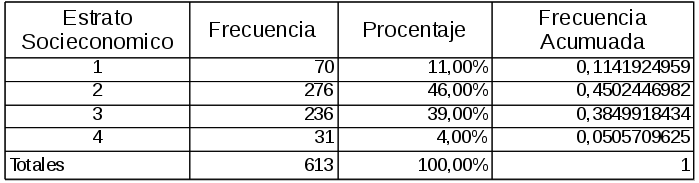
\includegraphics[width=0.9\linewidth]{figure/cuadro_socioeconomico}
		\caption{Variable Estrato Socioeconomico}
		\label{fig:cuadro_socioeconomico}
	\end{figure}

	En la Figura 2 se representa gráficamente la población por estrato utilizando diagramas de sectores o torta:  
	\bigskip

	\begin{figure} [ht]
		\centering
		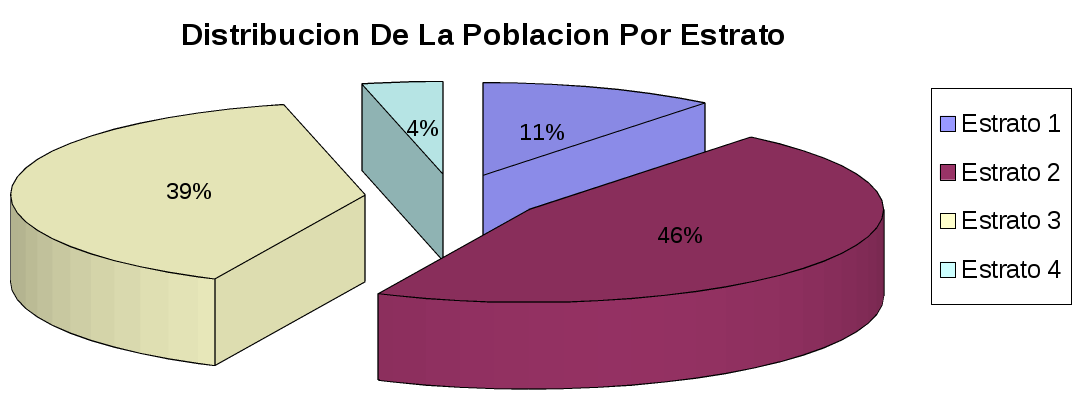
\includegraphics[width=0.9\linewidth]{figure/diagrama_sectores}
		\caption{Diagrama de sectores}
		\label{fig:diagrama_sectores}
	\end{figure}

	Como se puede observar en el diagrama de sectores la mayor cantidad de observaciones se encuentran agrupadas en el estrato 2 con un porcentaje de ocurrencia del 46\%.\\
	   
	Como se puede observar en el diagrama de barras de la Figura 3, la mayor cantidad de observaciones en la población ocurren en el estrato 2 con una frecuencia de 275 que corresponde al estrato hacia el que tienden a agruparsen las observaciones.
   
	\begin{figure}[ht]
		\centering
\begin{kframe}
\begin{alltt}
        \hlkwd{with}\hlstd{(datosep,} \hlkwd{hist}\hlstd{(estrato,} \hlkwc{breaks}\hlstd{=}\hlstr{"Sturges"}\hlstd{,} \hlkwc{col}\hlstd{=}\hlstr{"darkgray"}\hlstd{,} \hlkwc{main}\hlstd{=}\hlstr{"Diagrama de barras"}\hlstd{))}
\end{alltt}
\end{kframe}
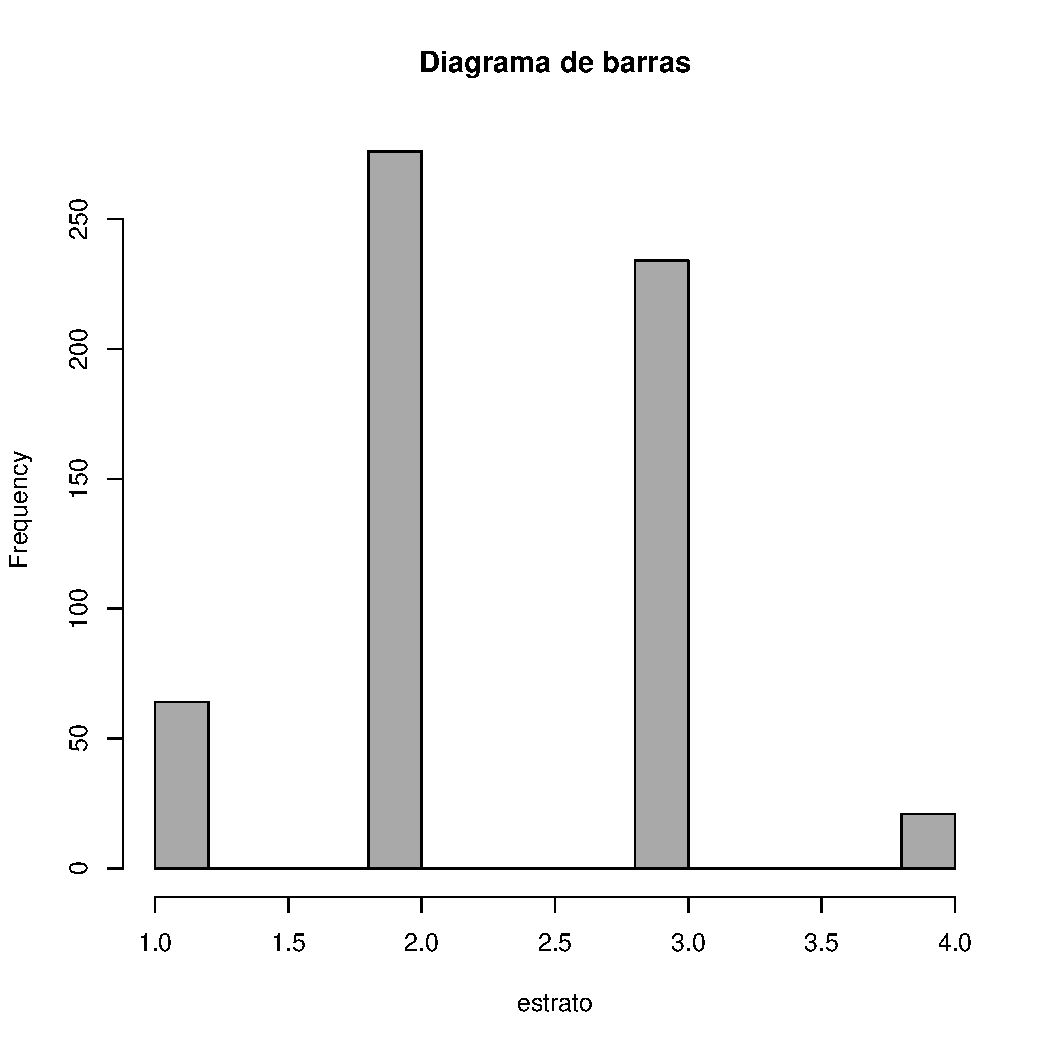
\includegraphics[width=\maxwidth]{figure/estrato-1} 

		\caption{Diagrama para estrato socioeconómico}
		\label{fig:diagrama_barras}
	\end{figure}

  	\item \textbf {Variable Promedio Ponderado de Carrera:}
	El promedio ponderado de carrera es una variable de carácter cuantitativo de tipo continuo, a la que se le puede aplicar la media y la mediana como medidas de tendencia central, a continuación se presentan los resultados.
	
\begin{kframe}
\begin{alltt}
        \hlstd{dfull} \hlkwb{<-} \hlkwd{data.frame}\hlstd{(}\hlkwc{Estrato}\hlstd{=datosep}\hlopt{$}\hlstd{estrato)}
        \hlkwd{stargazer}\hlstd{(dfull,} \hlkwc{type}\hlstd{=}\hlstr{"latex"}\hlstd{,} \hlkwc{title}\hlstd{=}\hlstr{"Promedio academico ponderado"}\hlstd{)}
\end{alltt}
\end{kframe}
% Table created by stargazer v.5.2 by Marek Hlavac, Harvard University. E-mail: hlavac at fas.harvard.edu
% Date and time: vie, jun 03, 2016 - 00:02:04
\begin{table}[!htbp] \centering 
  \caption{Promedio academico ponderado} 
  \label{} 
\begin{tabular}{@{\extracolsep{5pt}}lccccc} 
\\[-1.8ex]\hline 
\hline \\[-1.8ex] 
Statistic & \multicolumn{1}{c}{N} & \multicolumn{1}{c}{Mean} & \multicolumn{1}{c}{St. Dev.} & \multicolumn{1}{c}{Min} & \multicolumn{1}{c}{Max} \\ 
\hline \\[-1.8ex] 
Estrato & 595 & 2.356 & 0.718 & 1 & 4 \\ 
\hline \\[-1.8ex] 
\end{tabular} 
\end{table} 

	
	Se construyeron 5 intervalos de frecuencia de clase con el fin de facilitar el tratamiento y representación de los 613 promedios de carrera de los estudiantes de pregrado de la Universidad de los Llanos, los cuales se muestran a continuación:
	%\bigskip
	
	\begin{itemize}
		\item Intervalo 1: promedios de carrera entre 0 y 1  
		\item Intervalo 2: promedios de carrera entre 1,1 y 2
		\item Intervalo 3: promedios de carrera entre 2,1 y 3
		\item Intervalo 4: promedios de carrera entre 3,1 y 4 
		\item Intervalo 5: promedios de carrera entre 4,1 y 5
	\end{itemize}
%	\bigskip
		
	La tabla de frecuencias de la Figura 4 muestra el comportamiento de la variable promedio ponderado respecto a cada uno de los intervalos de clase.	
	
	\begin{figure}[ht]
		\centering
		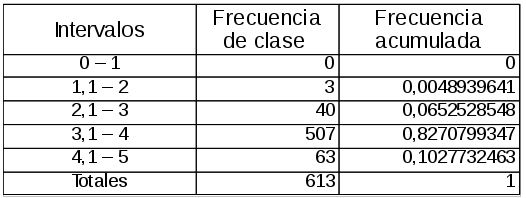
\includegraphics[width=0.7\linewidth]{figure/cuadro_promedio}
		\caption{Variable Promedio Ponderado de Carrera}
		\label{fig:cuadro_promedio}
	\end{figure}
	La Figura 5 representa gráficamente el comportamiento de la variable promedio ponderado de carrera mediante histograma de frecuencias de clases.

	\begin{figure}[ht]
		\centering
\begin{kframe}
\begin{alltt}
        \hlkwd{with}\hlstd{(datosep,} \hlkwd{hist}\hlstd{(promedio,} \hlkwc{breaks}\hlstd{=}\hlstr{"Sturges"}\hlstd{,} \hlkwc{col}\hlstd{=}\hlstr{"darkgray"}\hlstd{,} \hlkwc{main}\hlstd{=}\hlstr{"Histograma de frecuencias de clases"}\hlstd{))}
\end{alltt}
\end{kframe}
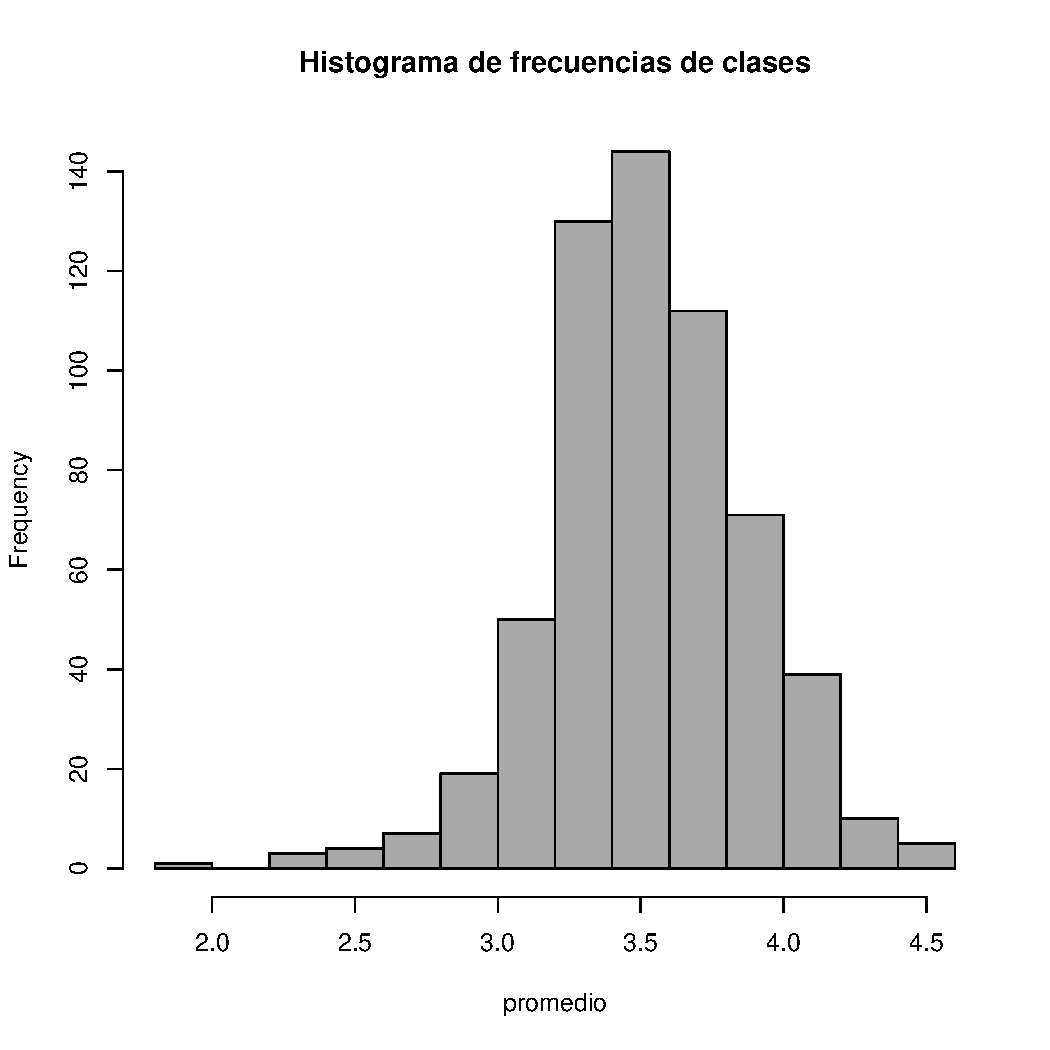
\includegraphics[width=\maxwidth]{figure/barrapromedio-1} 

		\caption{Histograma para Promedio Académico}
		\label{fig:barras_promedio_frecuencias_clase}
	\end{figure}

%	\begin{figure}[ht]
%		\centering
%		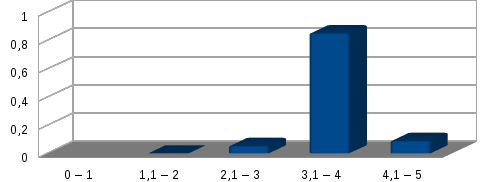
\includegraphics[width=0.9\linewidth]{figure/diagrama_barras_promedio}
%		\caption{Histograma Frecuencias Relativas}
%		\label{fig:diagrama_barras_promedio}
%	\end{figure}

	La Figura 6 muestra gráficamente la estimación de densidad para la variable promedio ponderado de carrera, lo que sugiere que los datos siguen una distribución normal y que se puede aplicar un estimador con base en la media o la varianza. 
	\begin{figure}[ht]
		\centering
\begin{kframe}
\begin{alltt}
        \hlkwd{densityplot}\hlstd{(} \hlopt{~} \hlstd{promedio,} \hlkwc{data}\hlstd{=datosep,} \hlkwc{bw}\hlstd{=}\hlstr{"SJ"}\hlstd{,} \hlkwc{adjust}\hlstd{=}\hlnum{1}\hlstd{,} \hlkwc{kernel}\hlstd{=}\hlstr{"epanechnikov"}\hlstd{,}  \hlkwc{main}\hlstd{=}\hlstr{"Diagrama de estimación de densidad"}\hlstd{)}
\end{alltt}
\end{kframe}
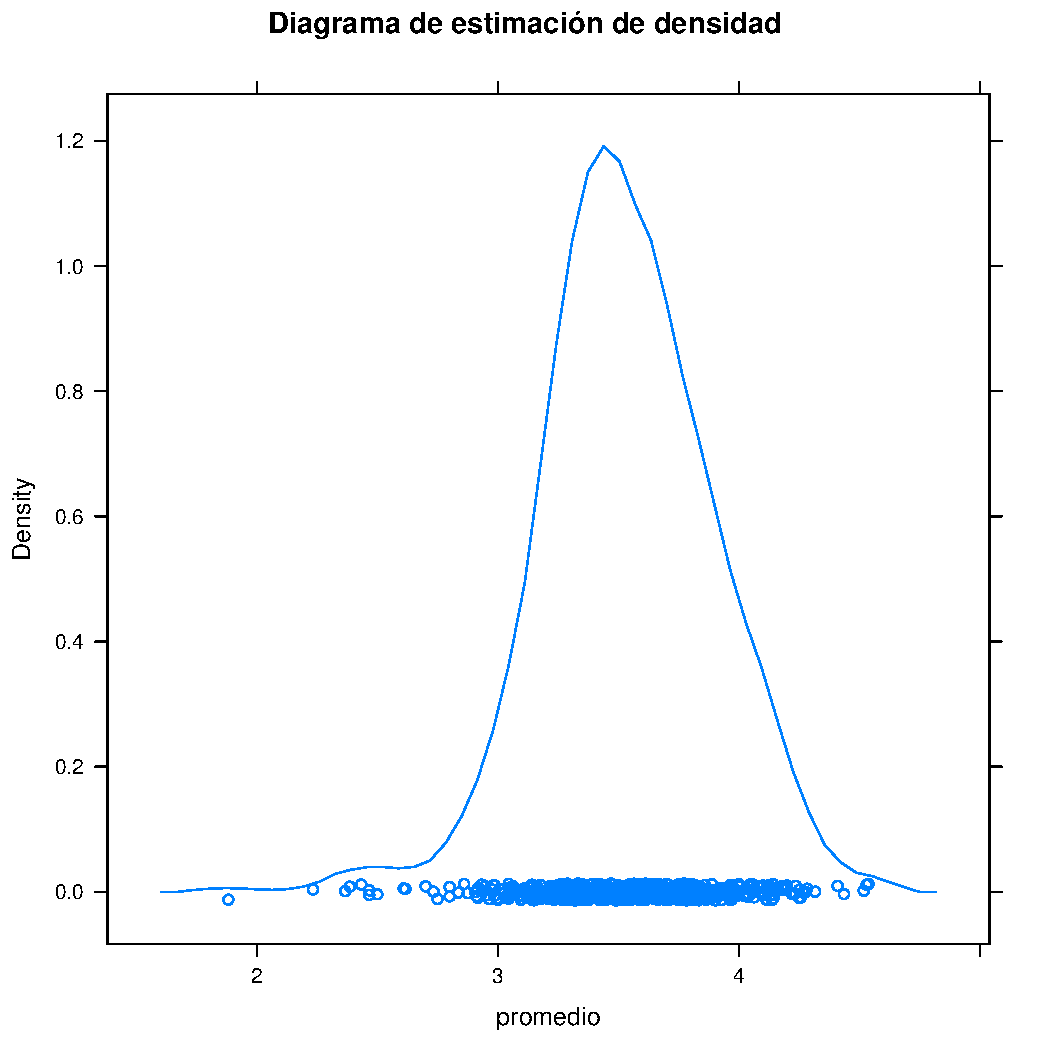
\includegraphics[width=\maxwidth]{figure/densidad-1} 
\begin{kframe}\begin{alltt}
        \hlcom{#densityplot( ~ promedio, data=datosep, bw="SJ", adjust=1, kernel="biweight")}
        \hlcom{#densityplot( ~ promedio, data=datosep, bw="SJ", adjust=1, kernel="gaussian")}
\end{alltt}
\end{kframe}
		\caption{Estimación de densidad para Promedio Académico}
		\label{fig:estimacion_frecuencia:promedio}
	\end{figure}

	\begin{figure}[ht]
		\centering
\begin{kframe}
\begin{alltt}
        \hlkwd{stripchart}\hlstd{(datosep}\hlopt{$}\hlstd{promedio,} \hlkwc{method}\hlstd{=}\hlstr{"stack"}\hlstd{,} \hlkwc{xlab}\hlstd{=}\hlstr{"Promedio ponderado Academico"}\hlstd{,} \hlkwc{main}\hlstd{=}\hlstr{"Diagrama de caja"}\hlstd{)}
\end{alltt}
\end{kframe}
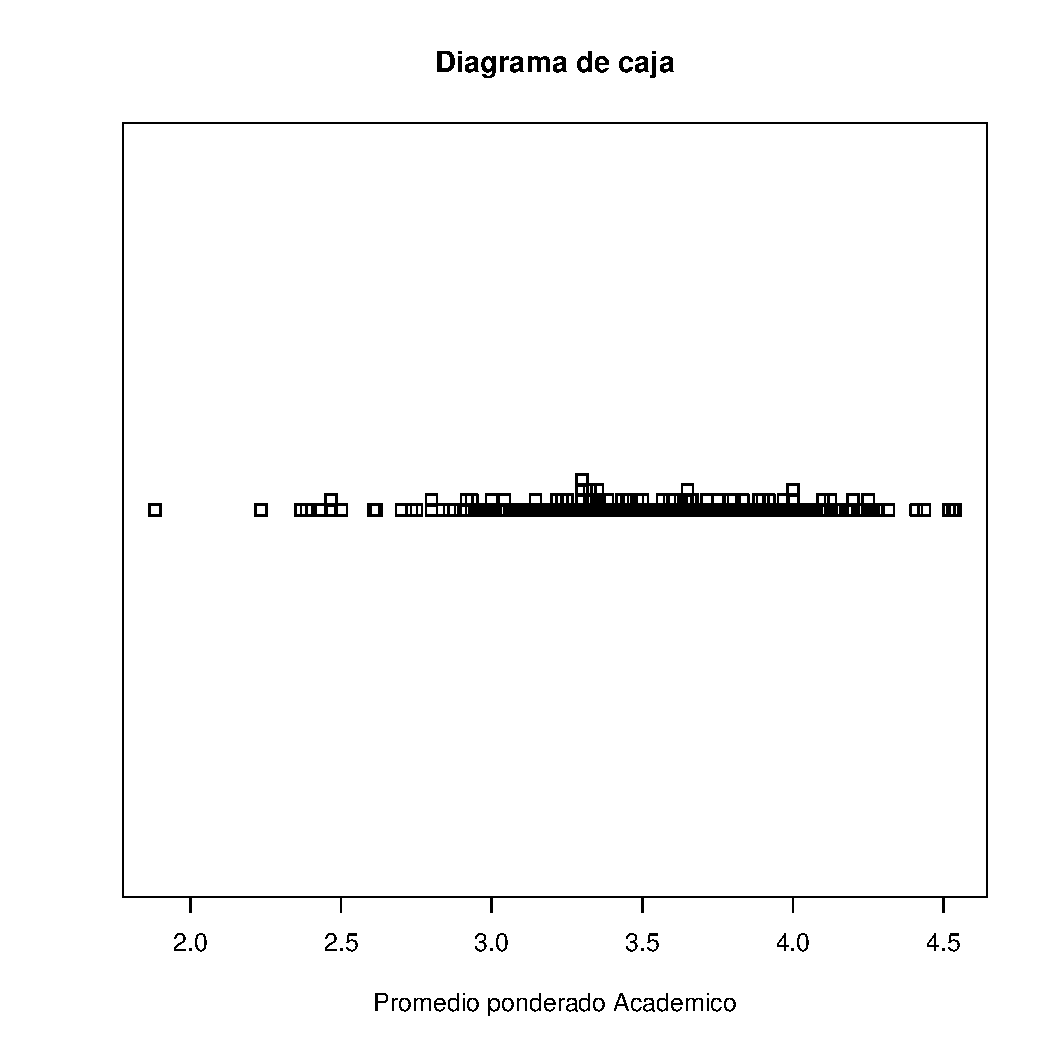
\includegraphics[width=\maxwidth]{figure/diagrama_puntos-1} 

		\caption{Diagrama de puntos para Promedio Académico}
		\label{fig:diagrama_puntos}
	\end{figure}

	Al aplicar la prueba de Shapiro-Wilk para validar el comportamiento de normal de los datos, se obtiene una confianza de W=0,9857 y p-value 0,0001457, como el valor de confianza deseado es 0,05 y el valor obtenido es menor se afirma que los datos no se comportan de forma normal.
	
	\begin{center}
		\bigskip
\begin{kframe}
\begin{alltt}
        \hlkwd{with}\hlstd{(datosep,} \hlkwd{shapiro.test}\hlstd{(promedio))}
\end{alltt}
\end{kframe}
	Shapiro-Wilk normality test

data:  promedio
W = 0.9857, p-value = 1.457e-05


	\end{center}
			
	\bigskip
	La Figura 7 muestra el diagrama de caja (box plot) que se construyo para visualizar gráficamente los datos atípicos que impiden que los datos alcancen el comportamiento normal.
		
	\begin{figure}[ht]
		\centering
\begin{kframe}
\begin{alltt}
        \hlkwd{boxplot}\hlstd{(datosep}\hlopt{$}\hlstd{promedio,} \hlkwc{data}\hlstd{=datosep,} \hlkwc{xlab}\hlstd{=}\hlstr{"Promedio Ponderado Academico"}\hlstd{,} \hlkwc{ylab}\hlstd{=}\hlstr{"Rango de calificación"}\hlstd{,} \hlkwc{id.method}\hlstd{=}\hlstr{"y"}\hlstd{,} \hlkwc{main}\hlstd{=}\hlstr{"Diagrama de caja"}\hlstd{)}
\end{alltt}
\end{kframe}
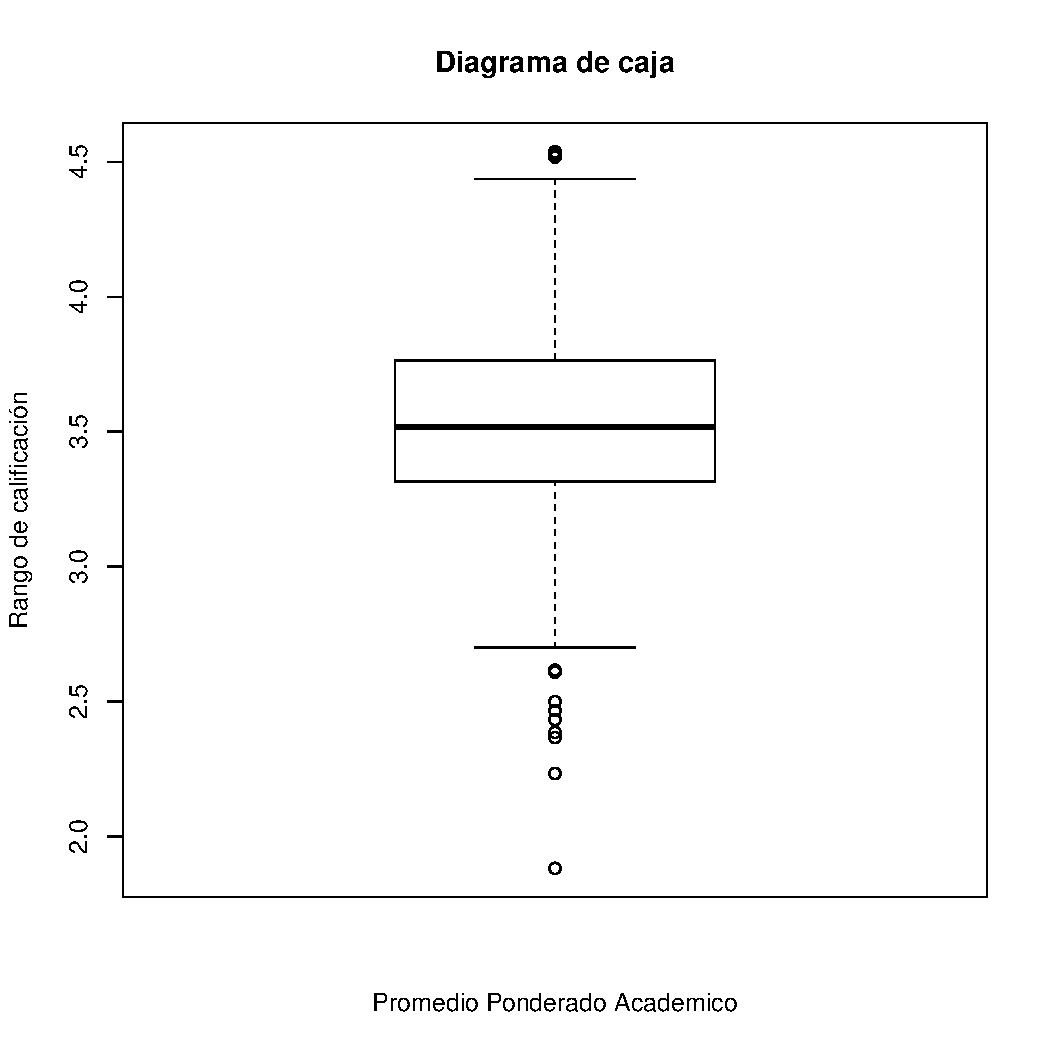
\includegraphics[width=\maxwidth]{figure/boxplot-1} 

		\caption{Diagrama de caja de la variable promedio}
		\label{fig:diagrama_boxplot_promedio}
	\end{figure}
	
	\bigskip

	Se aplica la técnica de truncamiento para forzar que los datos se comporten de forma normal, para ello se ordenan los datos de mayor a menor y se eliminan 150 datos, 75 en cada extremo. \\
	
	Se aplica nuevamente la prueba de normalidad de Shapiro-Wilk, obteniendo esta vez un comportamiento de normalidad en los datos resultados:\\
	
	\begin{center}
\begin{kframe}
\begin{alltt}
        \hlkwd{with}\hlstd{(datosept,} \hlkwd{shapiro.test}\hlstd{(promedio))}
\end{alltt}
\end{kframe}
	Shapiro-Wilk normality test

data:  promedio
W = 0.9857, p-value = 3.387e-05


	\end{center}
	\bigskip	
	Se realiza nuevamente el diagrama de caja (box plot) y se confirma que ya no existen datos outline o atípicos.
	
	\begin{figure}[ht]
		\centering
\begin{kframe}
\begin{alltt}
        \hlkwd{boxplot}\hlstd{(datosept}\hlopt{$}\hlstd{promedio,} \hlkwc{data}\hlstd{=datosept,} \hlkwc{xlab}\hlstd{=}\hlstr{"Promedio Ponderado Academico"}\hlstd{,} \hlkwc{ylab}\hlstd{=}\hlstr{"Rango de calificación"}\hlstd{,} \hlkwc{id.method}\hlstd{=}\hlstr{"y"}\hlstd{,} \hlkwc{main}\hlstd{=}\hlstr{"Diagrama de caja"}\hlstd{)}
\end{alltt}
\end{kframe}
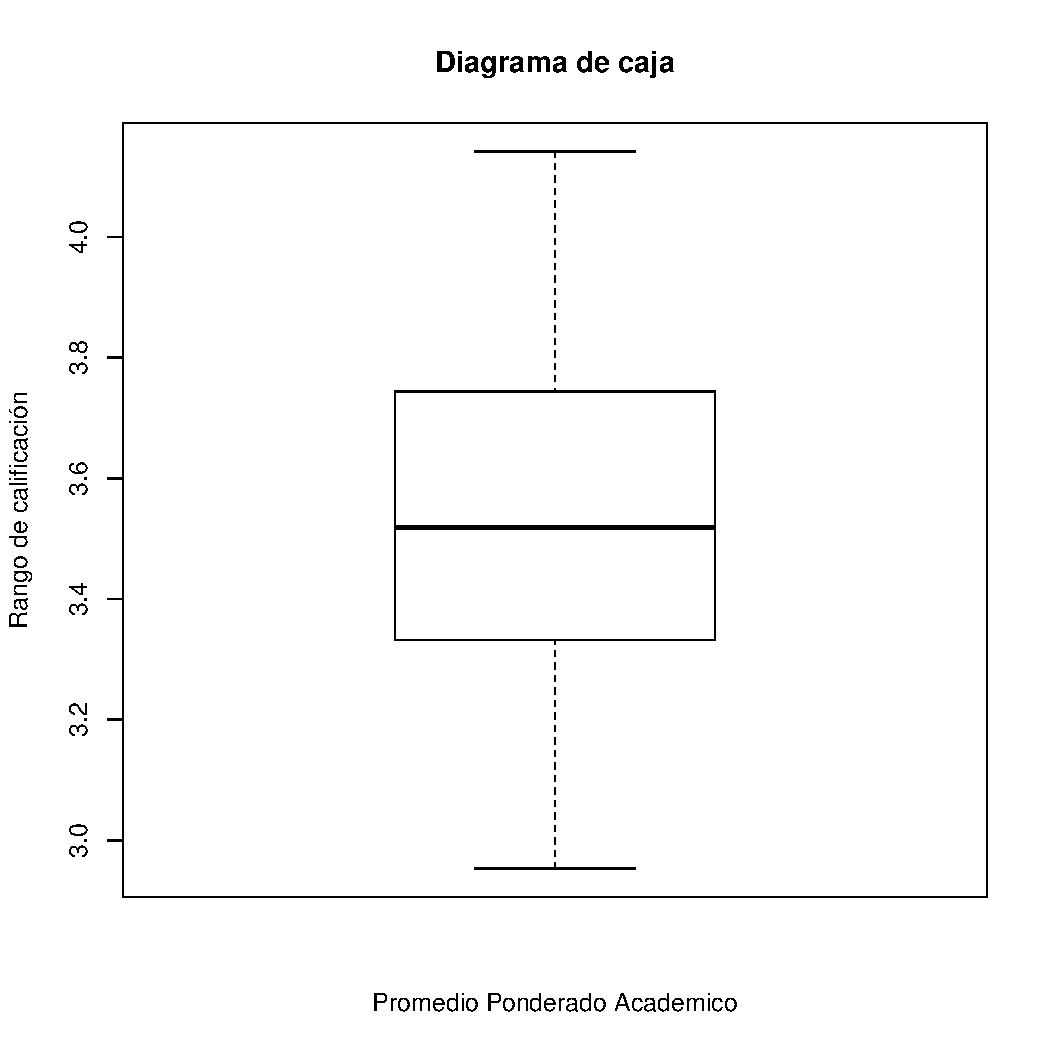
\includegraphics[width=\maxwidth]{figure/boxplot_trucado-1} 

		\caption{Diagrama de caja de la variable promedio truncada}
		\label{fig:diagrama_boxplot_promedio_truncada}
	\end{figure}
		
	\begin{figure}[ht]
		\centering
\begin{kframe}
\begin{alltt}
        \hlcom{#xyplot(promedio ~ estrato, type="p", pch=16, auto.key=list(border=TRUE), par.settings=simpleTheme(pch=16), scales=list(x=list(relation='same'), y=list(relation='same')), data=datosep)}

        \hlcom{#scatterplot(datosep$promedio~datosep$estrato, reg.line=lm, smooth=TRUE, spread=TRUE, id.method='mahal', id.n = 2, boxplots='xy', span=0.5, data=datosep, main="Estimación de densidad")}

        \hlcom{#scatterplot(promedio~estrato, reg.line=lm, smooth=TRUE, spread=TRUE, id.method='mahal', id.n = 2, boxplots='xy', span=0.5, data=datosep, main="Estimación de densidad")}

        \hlkwd{ggplot}\hlstd{(datosep,}\hlkwd{aes}\hlstd{(TPH),}\hlkwd{label}\hlstd{(}\hlstr{""}\hlstd{))} \hlopt{+} \hlkwd{geom_dotplot}\hlstd{()}
\end{alltt}


{\ttfamily\noindent\bfseries\color{errorcolor}{\#\# Error in eval(expr, envir, enclos): objeto 'TPH' no encontrado}}\end{kframe}
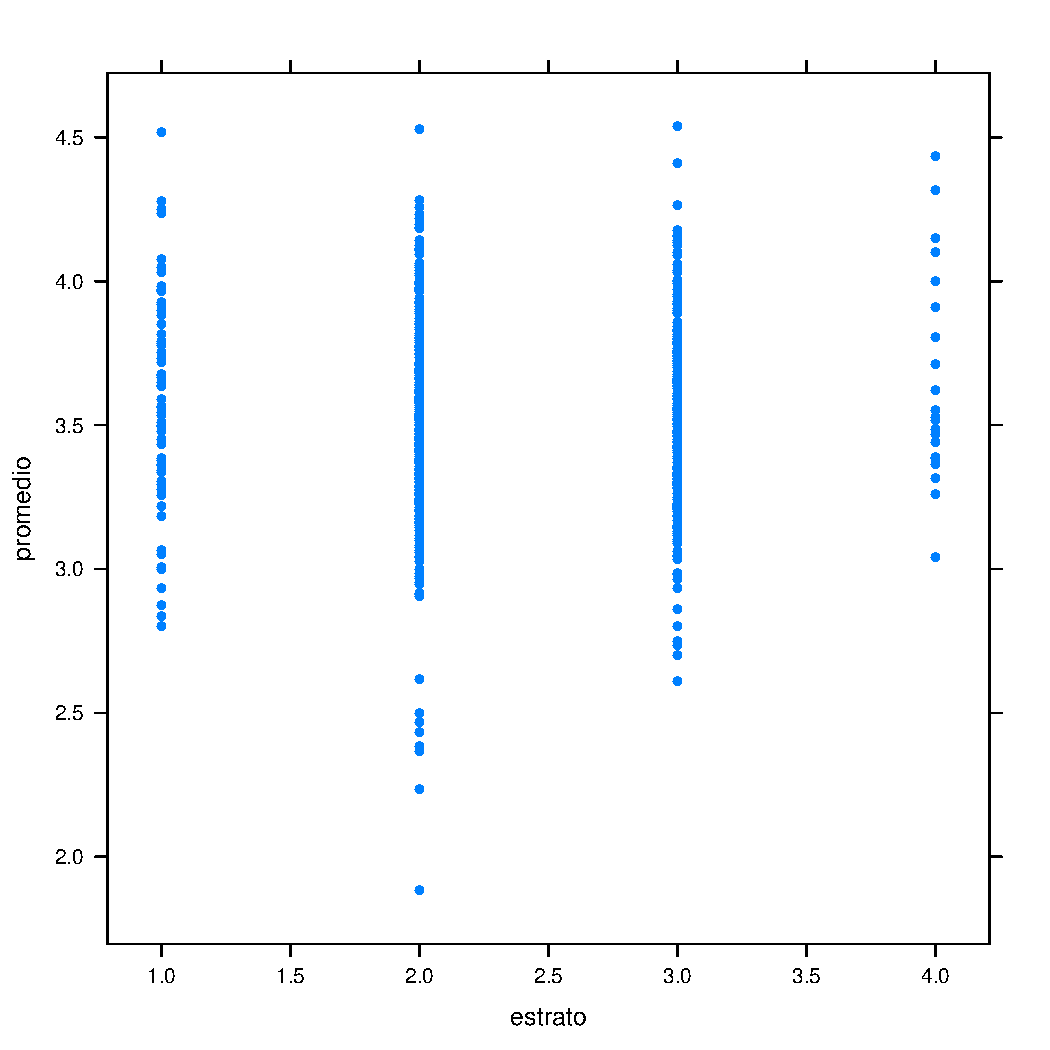
\includegraphics[width=\maxwidth]{figure/dispersion-1} 

		\caption{Diagrama de dispersión}
		\label{fig:diagrama_dispersion}
	\end{figure}
	
	\item \textbf {Diseño del espacio muestral:}
	El muestreo aplicado para abordar el análisis del dataset es Muestreo Aleatorio Simple (MAS) y el método utilizado para realizar la selección de los datos que conforman la muestra es coordinado negativo, a continuación se relacionan los cálculos realizados para obtener el tamaño de la muestra:
	\bigskip
	\begin{itemize}
		\item Asignar un numero aleatorio a cada dato de la muestra
		\item Ordenar de menor a mayor, de acuerdo al dato aleatorio cada elemento de la muestra
		\item Seleccionar desde primer dato hasta el tamaño de la muestra
	\end{itemize}
	\bigskip
	Los datos introducidos en los parámetros que proporciona la plantilla (documento adjunto) para calcular el tamaño de la muestra utilizando Muestreo Aleatorio Simple MAS, son los que se muestran a continuación:\\
	
	\begin{itemize}
		\item Tamaño de la población 	N = 5000	
		\item Error que se comete		E = 0,03	\\se recomienda que este entre 0,02 y 0,03
		\item Proporción del dominio	P = 0,30	\\P tomar valores entre 0 y 1
		\item Nivel de confianza		C = 0,91	\\(1 – alfa) donde alfa toma valores entre (0 y 1)
	\end{itemize}
	\bigskip
  	  	El tamaño de la muestra después de aplicar la técnica del coordinador negativo (M) es:
  	\bigskip  	
  	\begin{itemize}
  		\item Variabilidad			V = 0,2100420084
	  	\item Valor del percentil 	Z(alfa) = -1,6953977103
		\item Tamaño de la muestra 	M = 591  	
  	\end{itemize}
  	\bigskip  	
  	Una vez obtenido el tamaño de la muestra, se aplico la técnica de coordinador negativo a los datos de los estudiantes; el procedimiento realizado es el que se describe a continuación:
  	\bigskip
  	\begin{itemize}
  		\item Asigna un numero aleatorio a cada dato de la muestra
		\item Se ordena de menor a mayor con respecto a la asignación aleatoria 
		\item Se selecciona del primero hasta el tamaño de la muestra  
  	 \end{itemize}
  	\bigskip  		
  	Para el caso de los estudiantes de la Universidad de los Llanos se poseen los datos completos de toda la población objeto de análisis, pero con fin de corroborar la valides de los datos proporcionados mediante una encuesta, se calcula el tamaño de la muestra y se realiza la estimación bajo criterios de normalidad se selecciono una muestra de tamaño 613.
  	  	
   
  % \item Medidas de tendencia central[4] 
		 %15\
		 %\item Varianza [4] : La Varianza de las observaciones %$x_{1},x_{2},...,x_{n}$ es en esencia, el promedio del cuadrado %de las distancias entre cada observaci\'on y la media del %conjunto de observaciones. Se denota por:
		 %$$s^{2}=\sum_{i=1}^{n} \frac{ \left( %x_{i}-\overline{x}\right)^{2}}{\left(n-1 \right) } $$ 
		 
		 %\item Desviación estándar [4]: La desviaci\'on est\'andar es la %raiz cuadrada de la varianza y se denota por:
		 %$$s=\sqrt{\sum_{i=1}^{n} \frac{ \left( %x_{i}-\overline{x}\right)^{2}}{\left(n-1 \right) } }$$ 
		 		 
		 %Se puede aplicar una medida de tendencia central como la media y %un medida de dispersión  como la varianza. A continuación se %muestran los valores calculados para la variable promedio de %carrera ponderado.
%		 \begin{figure}[ht]
%			\centering
%			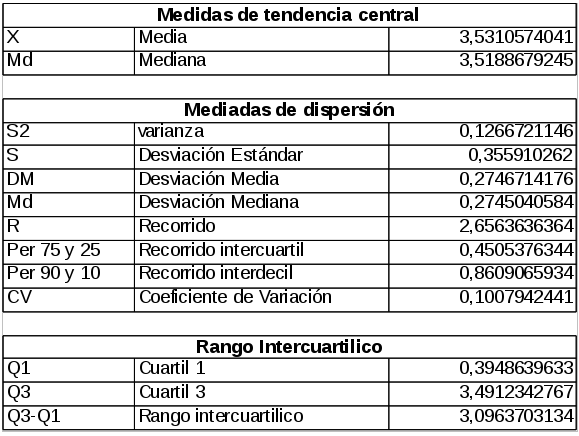
\includegraphics[width=0.9\linewidth]{figure/medidas_rpbabilidad}
%			\caption{}
%			\label{fig:medidas_rpbabilidad}
%		\end{figure}
 
\end{itemize} 

%SECCIÓN 3. PREGUNTAS INVESTIGACION
\section{Information Recognizing}
In this section will be described the data domain, the dataset, and the variables recognizing, and the SMART objectives.

 \subsection{The domain of the data.}
 One of the common uses of the business intelligence is oriented to the marketing, because all the organizations needs to know the current state of them, the history of their behavior, the capacity to satisfy the client requests and to increase their competitive.\\
 In this data analysis the dataset used is provided by  \href{http://archive.ics.uci.edu/ml/datasets/Online+Retail}{UCI on the official web site} and it contains some records related with the transactions of a store through a time period.
 \subsection{The Dataset}
  Like the UCI web page says, the dataset contains all the transactions occurring between 01/12/2010 and 09/12/2011 for a UK-based and registered non-store online retail.The company mainly sells unique all-occasion gifts. Many customers of the company are wholesalers, it's made off 541909 records of online retails and is composed by a the next fields.
 \begin{itemize}
  \item{InvoiceNo.} Invoice number. Nominal, a 6-digit integral number uniquely assigned to each transaction. If this code starts with letter 'c', it indicates a cancellation. 
  \item{StockCode.} Product (item) code. Nominal, a 5-digit integral number uniquely assigned to each distinct product. 
  \item{Description.} Product (item) name. Nominal. 
  \item{Quantity.} The quantities of each product (item) per transaction. Numeric.	
  \item{InvoiceDate.} Invoice Date and time. Numeric, the day and time when each transaction was generated. 
  \item{UnitPrice.} Unit price. Numeric, Product price per unit in sterling. 
  \item{CustomerID.} Customer number. Nominal, a 5-digit integral number uniquely assigned to each customer. 
  \item{Country.} Country name. Nominal, the name of the country where each customer resides.
 \end{itemize}
 \subsection{Smart Objectives}
 Check the behavior of the online retails from the past, to establish patterns, tendencies, and behaviors of the market.\\
 This objective must be the of high quality because the stakeholder may use it to take decisions.






  

  

  

  

  

  

  
    


%SECCIÓN 3. PREGUNTAS INVESTIGACION
\section{Research Questions}
A correct investigation begins with the right questions, then an optimal definition of what else will be the proposal of the research. The following questions are used in this research, these questions must be classified according with the kind of it.

  \subsection{Descriptive.}
  A descriptive question is used to identify and know the characteristics of the dataset.
  \begin{itemize}
   \item What's the min date of the measurement?
\begin{knitrout}
\definecolor{shadecolor}{rgb}{0.969, 0.969, 0.969}\color{fgcolor}\begin{kframe}
\begin{verbatim}
## [1] "2010-12-01"
\end{verbatim}
\end{kframe}
\end{knitrout}
   \item What's the max date of the measurement?
\begin{knitrout}
\definecolor{shadecolor}{rgb}{0.969, 0.969, 0.969}\color{fgcolor}\begin{kframe}
\begin{verbatim}
## [1] "2011-12-09"
\end{verbatim}
\end{kframe}
\end{knitrout}
   \item What's the product quantity sold in the measurement?
\begin{knitrout}
\definecolor{shadecolor}{rgb}{0.969, 0.969, 0.969}\color{fgcolor}\begin{kframe}
\begin{verbatim}
## [1] 5660981
\end{verbatim}
\end{kframe}
\end{knitrout}
   \item What's the product quantity returned in the measurement?
\begin{knitrout}
\definecolor{shadecolor}{rgb}{0.969, 0.969, 0.969}\color{fgcolor}\begin{kframe}
\begin{verbatim}
## [1] 484531
\end{verbatim}
\end{kframe}
\end{knitrout}
  \end{itemize}
  \subsection{Exploratory.}
   An exploratory question consists in the searching of patterns or relations to support an investigation question.
  \begin{itemize}
   \item Which month had major product sales and devolutions?
\begin{knitrout}
\definecolor{shadecolor}{rgb}{0.969, 0.969, 0.969}\color{fgcolor}
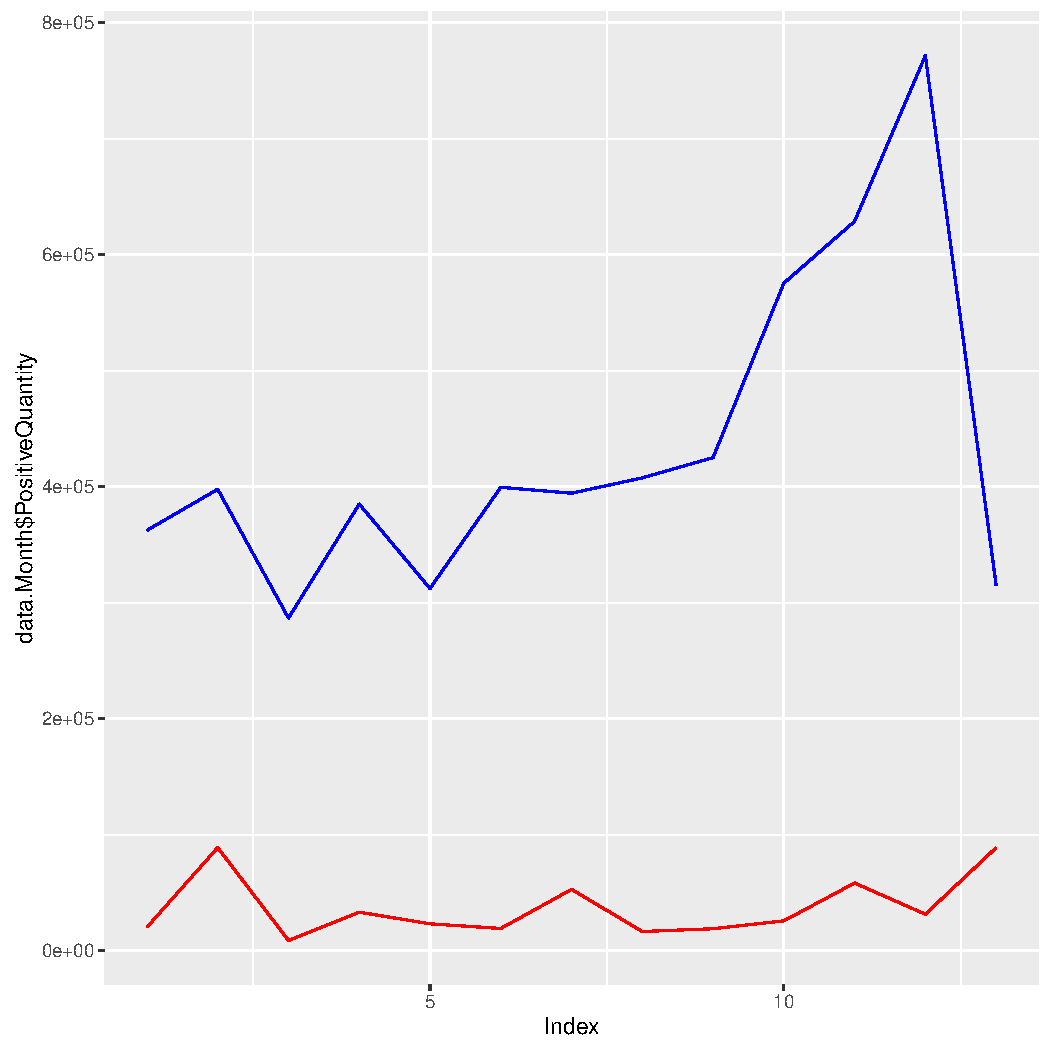
\includegraphics[width=\maxwidth]{figure/monthMajorSalesDevolutionsQuantity-1} 

\end{knitrout}

% latex table generated in R 3.3.0 by xtable 1.8-2 package
% Sat May 28 14:51:01 2016
\begin{table}[ht]
\centering
\begin{tabular}{rrlrr}
  \hline
 & Index & YearMonth & PositiveQuantity & NegativeQuantity \\ 
  \hline
1 &   1 & 2010 - 12 & 362316.00 & 20088.00 \\ 
  42482 &   2 & 2011 - 1 & 397716.00 & 88750.00 \\ 
  77629 &   3 & 2011 - 2 & 286695.00 & 8706.00 \\ 
  105336 &   4 & 2011 - 3 & 384950.00 & 33078.00 \\ 
  142084 &   5 & 2011 - 4 & 312176.00 & 23078.00 \\ 
  172000 &   6 & 2011 - 5 & 399425.00 & 19034.00 \\ 
  209030 &   7 & 2011 - 6 & 394337.00 & 52714.00 \\ 
  245904 &   8 & 2011 - 7 & 407539.00 & 16423.00 \\ 
  285422 &   9 & 2011 - 8 & 425016.00 & 18817.00 \\ 
  320706 &  10 & 2011 - 9 & 575416.00 & 25599.00 \\ 
  370932 &  11 & 2011 - 10 & 628745.00 & 58213.00 \\ 
  431674 &  12 & 2011 - 11 & 771598.00 & 31312.00 \\ 
  516385 &  13 & 2011 - 12 & 315052.00 & 88719.00 \\ 
   \hline
\end{tabular}
\caption{Dataset of product sales and devolution} 
\end{table}

   \item Which country bought the major products quantity in January of 2011?

% latex table generated in R 3.3.0 by xtable 1.8-2 package
% Sat May 28 14:51:01 2016
\begin{table}[ht]
\centering
\begin{tabular}{rlrrr}
  \hline
 & Country & PositiveQuantity & NegativeQuantity & Index \\ 
  \hline
44153 & Bahrain & 0.00 & 54.00 &   1 \\ 
  47164 & Japan & 0.00 & 45.00 &   2 \\ 
  50792 & Israel & 100.00 & 0.00 &   3 \\ 
  54381 & Cyprus & 144.00 & 0.00 &   4 \\ 
  72851 & Channel Islands & 259.00 & 4.00 &   5 \\ 
  58992 & Poland & 288.00 & 0.00 &   6 \\ 
  72247 & Iceland & 315.00 & 0.00 &   7 \\ 
  72986 & Lebanon & 386.00 & 0.00 &   8 \\ 
  69008 & Greece & 526.00 & 0.00 &   9 \\ 
  66153 & Finland & 765.00 & 0.00 &  10 \\ 
  43858 & Belgium & 792.00 & 9.00 &  11 \\ 
  70759 & Singapore & 1091.00 & 0.00 &  12 \\ 
  43780 & Italy & 1121.00 & 25.00 &  13 \\ 
  69624 & Hong Kong & 1121.00 & 0.00 &  14 \\ 
  43781 & Portugal & 2094.00 & 16.00 &  15 \\ 
  62999 & Switzerland & 2993.00 & 0.00 &  16 \\ 
  43420 & Sweden & 3097.00 & 1.00 &  17 \\ 
  45623 & Spain & 3845.00 & 8.00 &  18 \\ 
  45512 & Australia & 5644.00 & 0.00 &  19 \\ 
  44295 & EIRE & 8794.00 & 106.00 &  20 \\ 
  44206 & Germany & 9077.00 & 171.00 &  21 \\ 
  43857 & France & 9199.00 & 44.00 &  22 \\ 
  57394 & Netherlands & 20417.00 & 0.00 &  23 \\ 
  42482 & United Kingdom & 325648.00 & 88267.00 &  24 \\ 
   \hline
\end{tabular}
\caption{Information of buys in January of 2011} 
\end{table}

   
   \item Which country had major sales and devolutions of products?
% latex table generated in R 3.3.0 by xtable 1.8-2 package
% Sat May 28 14:51:01 2016
\begin{table}[ht]
\centering
\begin{tabular}{rrlrr}
  \hline
 & Index & Country & PositiveQuantity & NegativeQuantity \\ 
  \hline
100811 &   1 & Saudi Arabia & 80.00 & 5.00 \\ 
  38314 &   2 & Bahrain & 314.00 & 54.00 \\ 
  395473 &   3 & RSA & 352.00 & 0.00 \\ 
  157300 &   4 & Brazil & 356.00 & 0.00 \\ 
  72986 &   5 & Lebanon & 386.00 & 0.00 \\ 
  168150 &   6 & European Community & 499.00 & 2.00 \\ 
  7987 &   7 & Lithuania & 652.00 & 0.00 \\ 
  103599 &   8 & Czech Republic & 671.00 & 79.00 \\ 
  217685 &   9 & Malta & 970.00 & 26.00 \\ 
  89571 &  10 & United Arab Emirates & 982.00 & 0.00 \\ 
  69008 &  11 & Greece & 1557.00 & 1.00 \\ 
  14939 &  12 & Iceland & 2458.00 & 0.00 \\ 
  164465 &  13 & USA & 2458.00 & 1424.00 \\ 
  119192 &  14 & Canada & 2763.00 & 0.00 \\ 
  152713 &  15 & Unspecified & 3300.00 & 0.00 \\ 
  6609 &  16 & Poland & 3684.00 & 31.00 \\ 
  31983 &  17 & Israel & 4409.00 & 56.00 \\ 
  69624 &  18 & Hong Kong & 4773.00 & 4.00 \\ 
  31465 &  19 & Austria & 4881.00 & 54.00 \\ 
  70759 &  20 & Singapore & 5241.00 & 7.00 \\ 
  29733 &  21 & Cyprus & 6361.00 & 44.00 \\ 
  7215 &  22 & Italy & 8112.00 & 113.00 \\ 
  20018 &  23 & Denmark & 8235.00 & 47.00 \\ 
  20001 &  24 & Channel Islands & 9491.00 & 12.00 \\ 
  34084 &  25 & Finland & 10704.00 & 38.00 \\ 
  7135 &  26 & Portugal & 16258.00 & 78.00 \\ 
  1237 &  27 & Norway & 19338.00 & 91.00 \\ 
  7280 &  28 & Belgium & 23237.00 & 85.00 \\ 
  9784 &  29 & Japan & 26016.00 & 798.00 \\ 
  6422 &  30 & Spain & 27951.00 & 1127.00 \\ 
  5321 &  31 & Switzerland & 30630.00 & 305.00 \\ 
  30079 &  32 & Sweden & 36083.00 & 446.00 \\ 
  198 &  33 & Australia & 84209.00 & 556.00 \\ 
  27 &  34 & France & 112104.00 & 1624.00 \\ 
  1110 &  35 & Germany & 119263.00 & 1815.00 \\ 
  1405 &  36 & EIRE & 147447.00 & 4810.00 \\ 
  386 &  37 & Netherlands & 200937.00 & 809.00 \\ 
  1 &  38 & United Kingdom & 4733819.00 & 469990.00 \\ 
   \hline
\end{tabular}
\caption{Global information about the countries consumption} 
\end{table}

   
  \end{itemize}
  \subsection{Inferential.}
   An inferential question consists in the creation of an hypothesis to be solved analyzing the information.
  \begin{itemize}
   \item Was France the country with major sales in January of 2011?\\
   The Table III suggest that United Kingdom had the major sales in January of 2011
  \end{itemize}


%SECCIÓN 3. PREGUNTAS INVESTIGACION
\section{Exploratory Analysis}
In this section was made an analysis in some scenarios to check the information related with the "frequencies" and the "central tendency measures"\\

 The following information contains the resume of the exploratory analysis of the variables through the measure period
% latex table generated in R 3.3.0 by xtable 1.8-2 package
% Sat May 28 14:51:01 2016
\begin{table}[ht]
\centering
\begin{tabular}{rlrrrrr}
  \hline
 & Variable & mean & min & max & var & sd \\ 
  \hline
1 & Year & 2010.92 & 2010.00 & 2011.00 & 0.07 & 0.27 \\ 
  2 & Month & 7.55 & 1.00 & 12.00 & 12.31 & 3.51 \\ 
  3 & Day & 15.02 & 1.00 & 31.00 & 75.07 & 8.66 \\ 
  4 & Sold & 10.45 & 0.00 & 80995.00 & 24115.74 & 155.29 \\ 
  5 & Returned & 0.89 & 0.00 & 80995.00 & 23424.97 & 153.05 \\ 
   \hline
\end{tabular}
\caption{Summary of main variables} 
\end{table}

 
 As you can see in the table, it's a general overview around the dataset because meeting the exploratory information of the data you can assume you know the data set.


%SECCIÓN 3. PREGUNTAS INVESTIGACION
\section{Multivariate Analysis}
In this section you'll find the correlation analysis of variables to check the importance of them. This analysis allows checking the influence of an attribute on other, this analysis is commonly used to discard any attribute if it isn't important for other attributes.\\
\begin{knitrout}
\definecolor{shadecolor}{rgb}{0.969, 0.969, 0.969}\color{fgcolor}
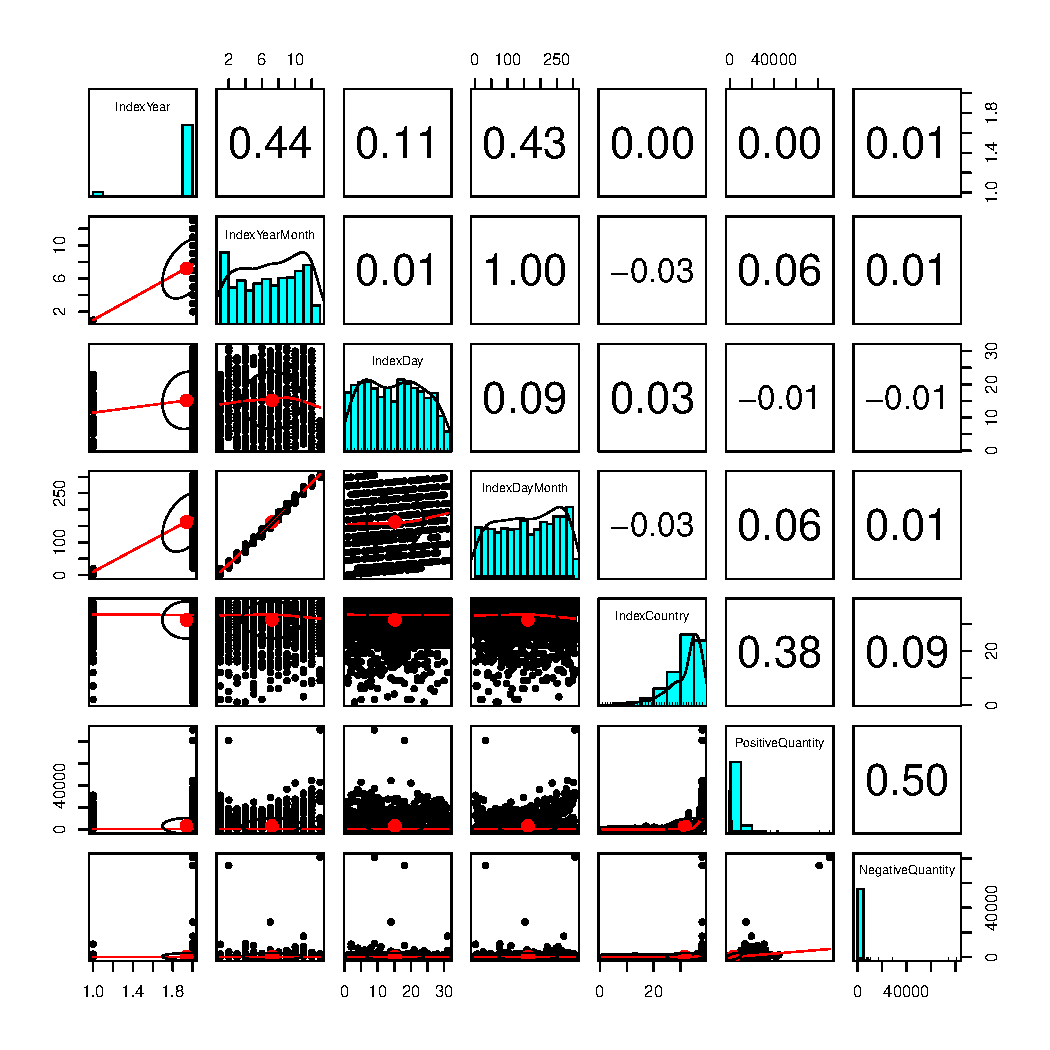
\includegraphics[width=\maxwidth]{figure/pairs-1} 

\end{knitrout}

As you can see in the previous chart we can think some conclusions like these
\begin{itemize}
 \item Applying the Pearson's correlation, we can discard the value related with the Country, because the correlation index is too near than 0
 \item The year and the month are some of the most important variables of the data analysis of this study.
 \item The Sales affects directly the Devolutions
\end{itemize}


%SECCIÓN 3. PREGUNTAS INVESTIGACION
\section{Finding Patterns}
In this section we are going to establish some patterns between the data using the linear regression algorithm and the K-means algorithm.\\
\subsection{Linear Regression}
This algorithm is used to build a model to reproduce the information drawing the nearest line to all the points.\\
For this dataset we'll use this algorithm in the relationship between the month days and the quantity.
\begin{knitrout}
\definecolor{shadecolor}{rgb}{0.969, 0.969, 0.969}\color{fgcolor}
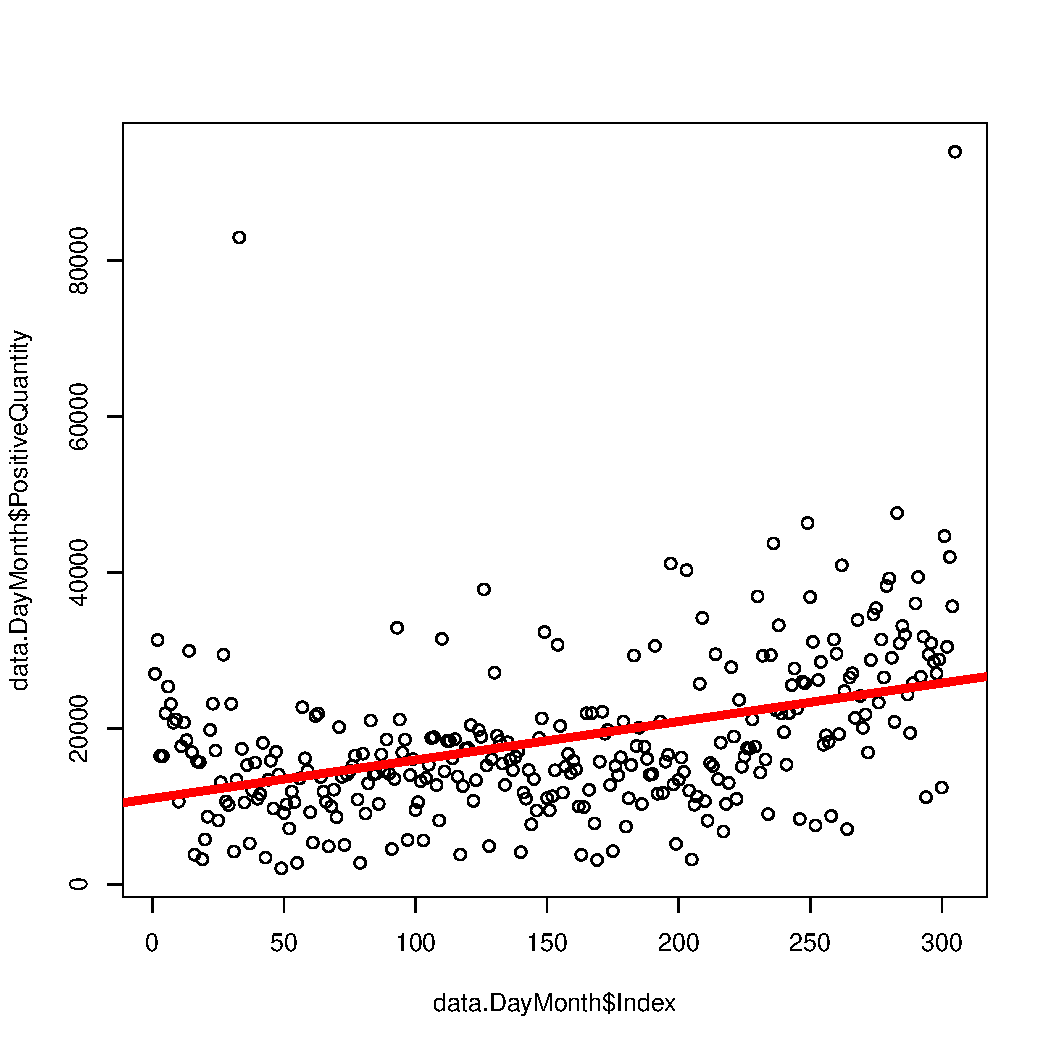
\includegraphics[width=\maxwidth]{figure/linear-regression-1} 

\end{knitrout}

\begin{knitrout}
\definecolor{shadecolor}{rgb}{0.969, 0.969, 0.969}\color{fgcolor}
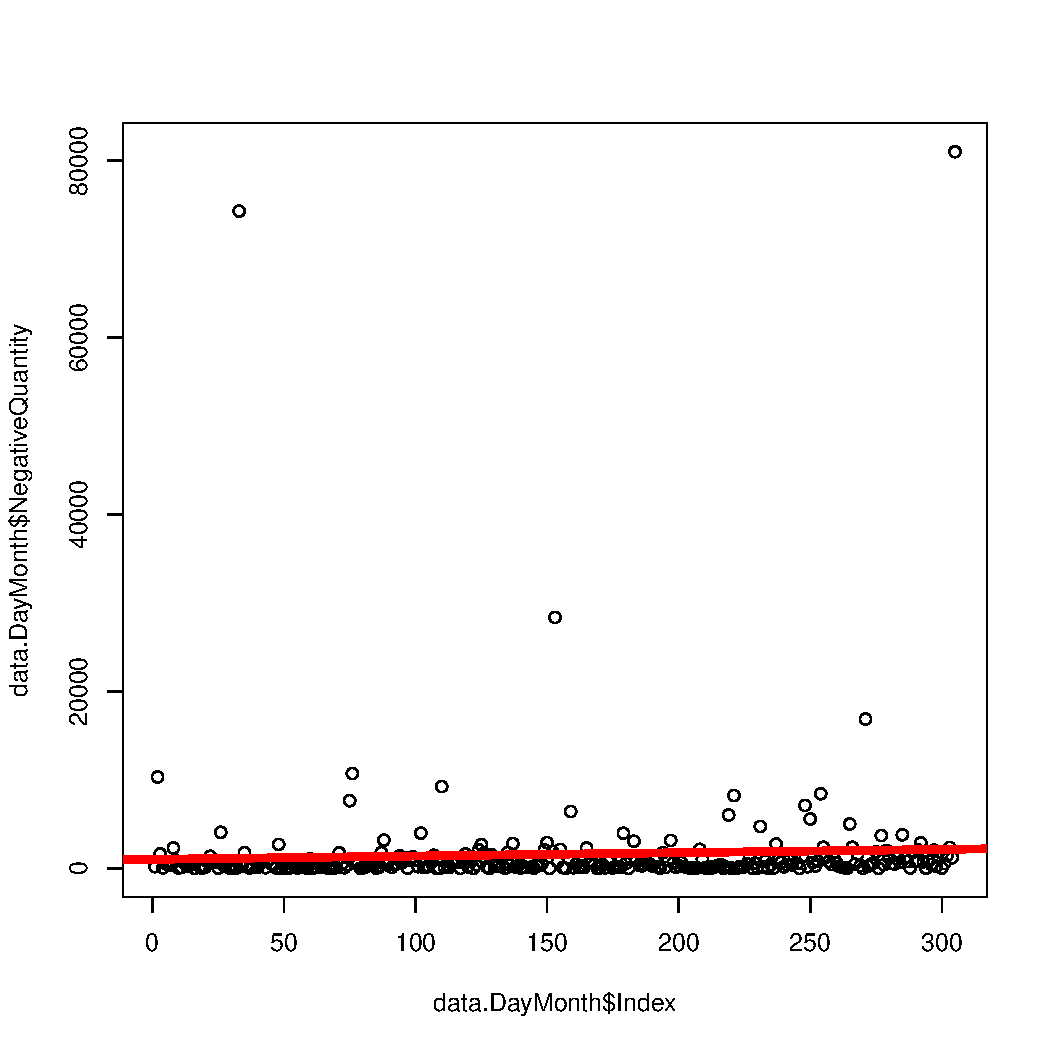
\includegraphics[width=\maxwidth]{figure/linear-regression2-1} 

\end{knitrout}

\subsection{Clustering}
This algorithm is used to build a model to reproduce the information drawing the nearest centroid to all the points of the cluster.\\
For this dataset we'll use this algorithm in the relationship between the months days and the quantity.

\begin{knitrout}
\definecolor{shadecolor}{rgb}{0.969, 0.969, 0.969}\color{fgcolor}
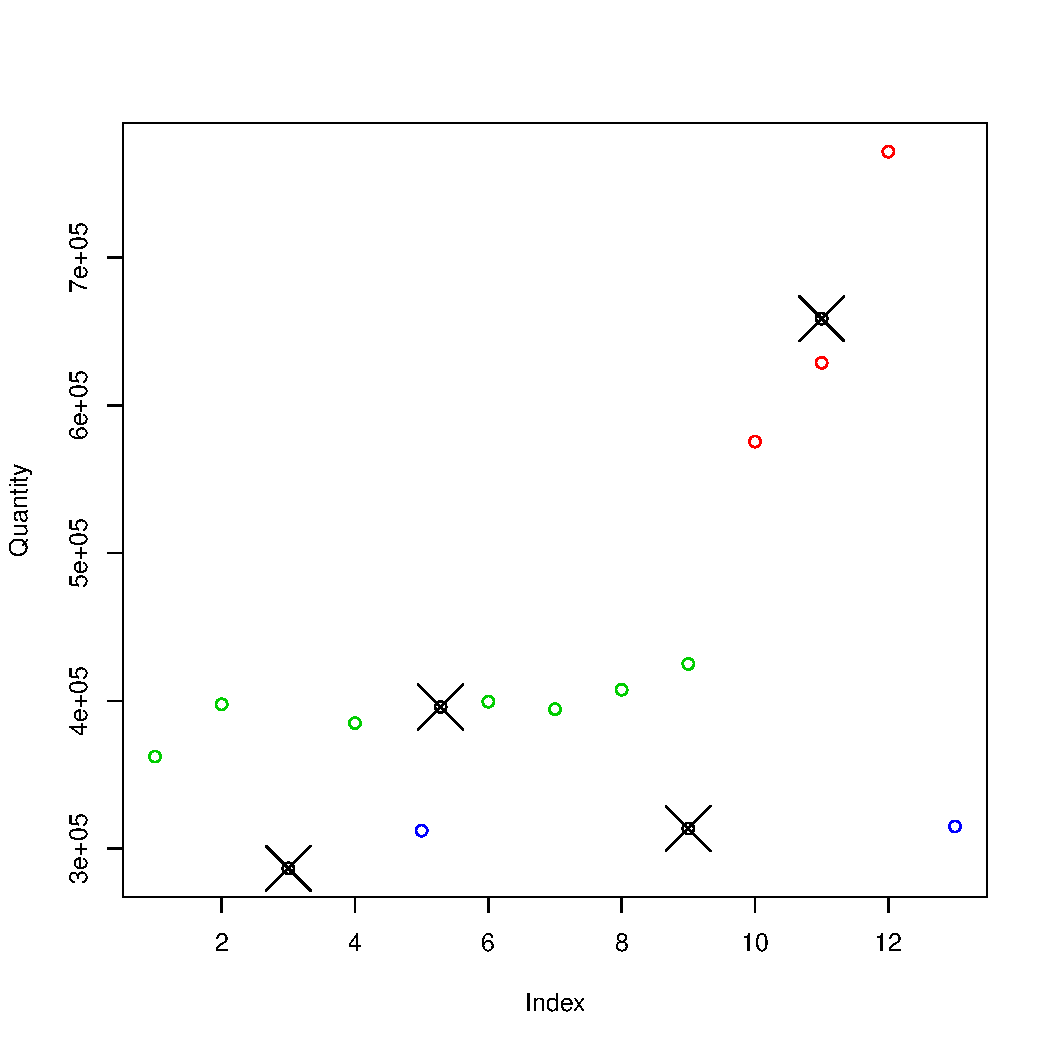
\includegraphics[width=\maxwidth]{figure/kmeans-1} 

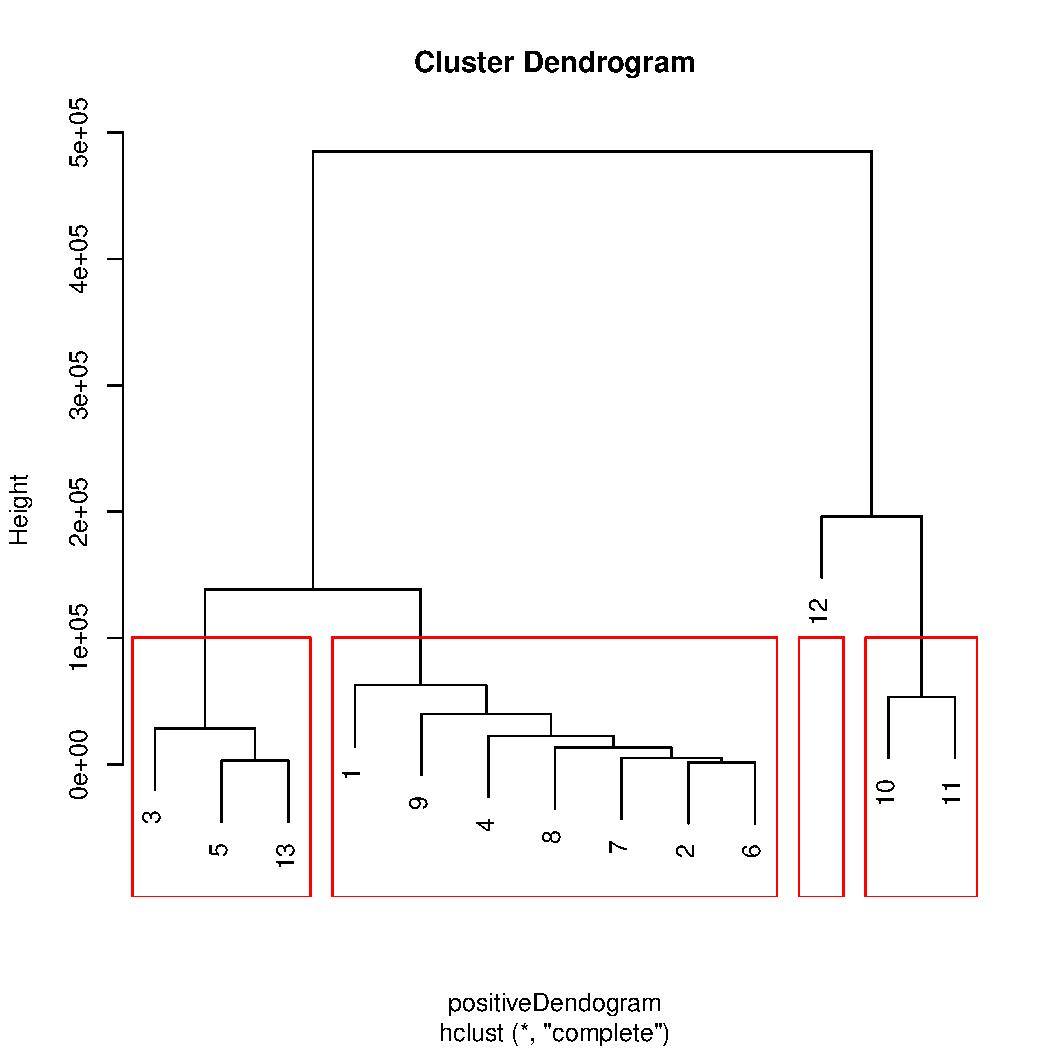
\includegraphics[width=\maxwidth]{figure/kmeans-2} 

\end{knitrout}




\section{Conclusions}
\begin{itemize}
 \item The data analysis of the dataset allows establishing some relationships and patterns to describe the behavior of the data.
 \item The critical task of the data analysis consists in understanding the dataset, the data preparation, and the tasks related with the patterns definition.
 \item The linear regression and the clustering using the K-means algorithm are good options to analyze some behaviors of the marketing.
 
 
\end{itemize}


%BIBLIOGRAFÍA

%ENTORNO {thebibliography}
%Permite al autor listar las referencias utilizadas y citarlas en algun punto del texto.

\begin{thebibliography}{1}
		
	\bibitem{biblio1} G. Canavos, Probabilidad y estadistica aplicaciones y metodos. Mc-Graw Hill, 1988. 
	\bibitem{biblio2} H. Chen, BUSINESS INTELLIGENCE AND ANALYTICS: FROM BIG DATA TO BIG IMPACT, MIS Quarterly Vol. 36 No. 4, pp. 1165-1188/December 2012 
	\bibitem{biblio3} Daqing Chen, Sai Liang Sain, and Kun Guo, Data mining for the online retail industry: A case study of RFM model-based customer segmentation using data mining, Journal of Database Marketing and Customer Strategy Management, Vol. 19, No. 3, pp. 197–208, 2012 
	\bibitem{biblio4} Ashishkumar Singh, Grace Rumantir, Annie South, Blair Bethwaite, Proceedings of the 2014 International Conference on Big Data Science and Computing.
	\bibitem{biblio5} A decision-making framework for precision marketing, Zhen You, Yain-Whar Si, Defu Zhang, XiangXiang Zeng, Stephen C.H. Leung c, Tao Li, Expert Systems with Applications, 42 (2015) 3357–3367.
	\bibitem{knitr-book} XIE, Yihui. Dynamic documents with R and knitr. Chapman \& Hall. Second edition. 2015.  
	\bibitem{latex-book} DE CASTRO KORGI, Rodrigo. El universo LATEX. Facultad de ciencias. Universidad Nacional de Colombia. Segunda edicion. 2003.  

\end{thebibliography}

\end{document}
